\documentclass{article}
\def\inputGnumericTable{}
\usepackage[utf8]{inputenc}
\usepackage{fullpage}
\usepackage{color}
\usepackage{array}
\usepackage{longtable}
\usepackage{calc}
\usepackage{multirow}
\usepackage{hhline}
\usepackage{ifthen}

% --- Required math + images + list packages (same as reference) ---
\usepackage{amsmath}
\usepackage{amsfonts}
\usepackage{amssymb}
\usepackage{graphicx}
\usepackage{enumitem}
\usepackage{float}

\begin{document}

% ==========================================
% HEADER BLOCK (Reference Style)
% ==========================================

\noindent
\begin{minipage}[t]{0.5\textwidth}
\vspace{0pt}

\includegraphics[width=5cm]{Logo.png}
\end{minipage}%
\begin{minipage}[t]{0.5\textwidth}
\vspace{0pt}
\begin{description}[font=\bfseries, style=multiline, leftmargin=3.5cm]
\item[Name:] Charan Kora
\item[ID:] COMETFWC049
\item[Date:] 30-01-26
\end{description}
\end{minipage}

\vspace{1cm}

\begin{center}
\textbf{\Large MATHEMATICS}
\end{center}

\hrule
\vspace{0.5cm}

% ==========================================
% SINGLE ENUMERATE LIST
% ==========================================

\section*{SECTION -- A}

\begin{enumerate}[label=\textbf{\arabic*.}, leftmargin=*, itemsep=1em]

\item In Fig., $PQ$ is a tangent at point $C$ to a circle.

\begin{figure}[H]
\centering
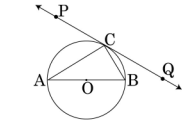
\includegraphics[width=0.6\linewidth]{1.png}
\end{figure}

\item For what value of $k$ will $k+9$, $2k-1$ and $2k+7$ be consecutive terms of an A.P.?

\item A ladder leaning against a wall makes an angle with the horizontal. Find its length.

\item A card is drawn at random from a well-shuffled pack of cards. Find the probability of the required event.

% ================= SECTION B =================

\item[]
\vspace{0.4cm}
\hrule
\vspace{0.2cm}
{\Large \textbf{SECTION -- B}}

\item If $-5$ is a root of the quadratic equation $2x^2 + px - 15 = 0$ and the quadratic equation $p(x^2 + x) + k = 0$ has equal roots, find $k$.

\item Let $P$ and $Q$ be the points of trisection of the line segment joining $A(2,-2)$ and $B(-7,4)$ such that $P$ is nearer to $A$. Find coordinates of $P$ and $Q$.

\item In Fig., a quadrilateral $ABCD$ circumscribes a circle. Prove that $AB + CD = BC + DA$.

\begin{figure}[H]
\centering
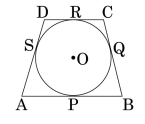
\includegraphics[width=0.6\linewidth]{2.png}
\end{figure}

\item Prove that the points $(3,0)$, $(6,4)$ and $(-1,3)$ form a right angled isosceles triangle.

\item The 4th term of an A.P. is zero. Prove that the 25th term is three times the 11th term.

\item From an external point $P$, two tangents are drawn to a circle. Show that $\angle OTS = \angle OST = 30^\circ$.

\begin{figure}[H]
\centering
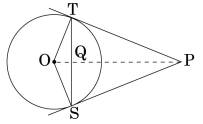
\includegraphics[width=0.6\linewidth]{3.png}
\end{figure}

% ================= SECTION C =================

\item[]
\vspace{0.4cm}
\hrule
\vspace{0.2cm}
{\Large \textbf{SECTION -- C}}

\item In Fig., $O$ is the centre of a circle such that required measurements are given. Find the area. Take $\pi = 3.14$.

\begin{figure}[H]
\centering
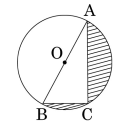
\includegraphics[width=0.6\linewidth]{4.png}
\end{figure}

\item A tent is in the shape of a cylinder surmounted by a cone. Find the canvas required. Use $\pi = \dfrac{22}{7}$.

\end{enumerate}

\end{document}
